\chapter{Software Process}
\label{chapter:SoftwareProcess}

An outstanding feature of ITK is the software process used to develop,
maintain, and test the toolkit. The Insight Toolkit software continues
to evolve rapidly due to the efforts of developers and users located around
the world, so the software process is essential to maintaining its
quality. If you are planning to contribute to ITK, or use the CVS source code
repository or the daily releases, you need to know something about this
process (see \ref{sec:ObtainingTheSoftware} on page 
\pageref{sec:ObtainingTheSoftware} to learn more about 
obtaining ITK using CVS). This information will help you know when and how to
update and work with the software as it changes. The following sections
describe key elements of the process.

\section{CVS Source Code Repository}
\label{sec:CVSRepository}

\index{ITK!CVS repository}
\index{CVS|textbf}

The Concurrent Versions System (CVS) is a tool for version control
\cite{Fogel1999}. It is a very valuable resource for software projects
involving multiple developers.  The primary purpose of CVS is to keep track
of changes to software. CVS date and version stamps every addition to the
repository---also providing for special user-specified tags---so that it is
possible to return to a particular state or point of time whenever
desired. The differences between any two points is represented by a ``diff''
file, that is a compact, incremental representation of change. CVS supports
concurrent development so that two developers can edit the same file at the
same time, that are then (usually) merged together without incident (and
marked if there is a conflict). In addition, branches off of the main
development trunk provide parallel development of software.

Developers and users can check out the software from the CVS repository. When
developers introduce changes in the system,  CVS facilitates to update the
local copies of other developers and users by downloading only the differences
between their local copy and the version on the repository.  This is an
important advantage for those who are interested in keeping up to date with the
leading edge of the toolkit. Bug fixes can be obtained in this way as soon as
they have been checked into the system.

ITK source code, data, and examples are maintained in a CVS repository.
The principal advantage of a system like CVS is that it frees developers to
try new ideas and changes without fear of losing a previous working version
of the software. It also provides a simple way to incrementally update code
as new features are added to the repository.



\section{DART Regression Testing System}
\label{sec:DART}
\label{sec:QualityDashboard}

\index{Dashboard|textbf}
\index{Quality Dashboard|textbf}
\index{Dart|textbf}

One of the unique features of the ITK software process is its use of the DART
regression testing system (\url{http://public.kitware.com/Dart}). In a
nutshell, what DART does is to provide quantifiable feedback to developers as
they check in new code and make changes. The feedback consists of the results
of a variety of tests, and the results are posted on a publically-accessible
Web page (to which we refer as a \emph{dashboard} as shown in Figure
\ref{fig:Dashboard} and accessible from
\url{http://www.itk.org/Testing/Dashboard/MostRecentResults-Nightly/Dashboard.html}).
All users and developers of ITK can view the dashboard, that produces
considerable peer-pressure on developers who check in code with problems. The
Dart dashboard serves as the vehicle for developer communication, and should
be viewed whenever you consider updating software via CVS or a daily release.

\begin{figure}[ht]
\centering 
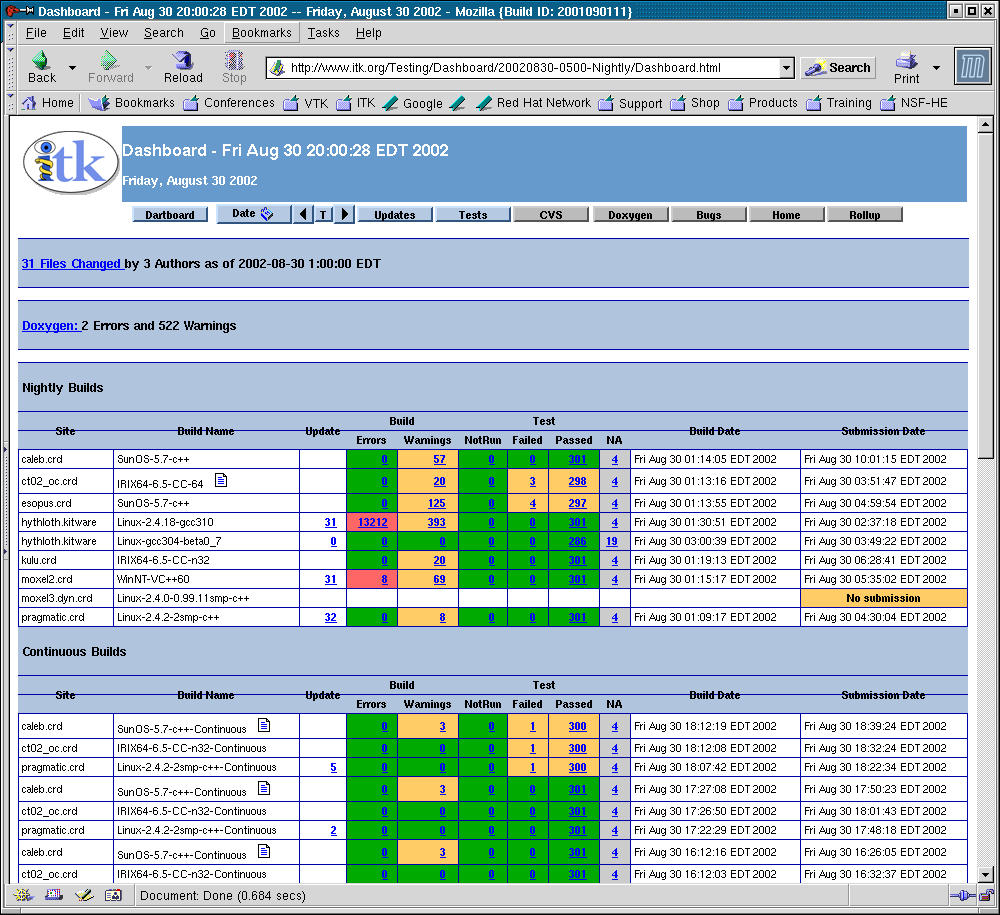
\includegraphics[width=0.7\textwidth]{Dashboard.eps}
\itkcaption[Dart Quality Dashboard]{On-line presentation of the Quality
Dashboard generated by Dart}
\label{fig:Dashboard}
\end{figure}

Note that DART is independent of ITK and can be used to manage quality
control for any software project. It is itself an open-source package and can
be obtained from

\begin{center} 
\url{http://public.kitware.com/Dart/HTML/Index.shtml}
\end{center} 

DART supports a variety of test types. These include the following.
\begin{description}
        \item[Compilation.] All source code is compiled and linked. Any
        resulting errors and warnings are reported.

        \item[Regression.] Most ITK tests produce images as output. Testing
        requires comparing each test�s output against a valid image. If
        the images match then the test passes. The comparison must be
        performed carefully since many 3D graphics systems (e.g., OpenGL)
        produce slightly different results on different platforms.

        \item[Memory.] One of the nastiest of problems to find in any
        computer program are those related to memory. Memory leakage,
        uninitialized memory, and reads and writes beyond allocated space are
        all examples of this sort of problem. ITK checks memory using Purify,
        a commercial package produced by Rational. (Other memory checking
        programs will be added in the future.)

        \item[PrintSelf.] All classes in ITK are expected to print out all
        their instance variables correctly. This test checks to make sure
        that this is the case.

        \item[SetGet.] Often developers make assumptions about the values of
        instance variables; i.e., they assume that they are non-NULL,
        etc. The SetGet tests perform a Get on all instance variables with a
        Get\_\_() method, followed by a Set method on the instance variable
        with the value returned from the Get\_\_() method. It's surprising
        how many times this test identifies problems.

        \item[TestEmptyInput.] This deceptively simple test catches many
        problems due to developers assuming that the input to a process
        object is non-NULL, or that the input data object contains some
        data. TestEmptyInput simply exercises these two conditions on each
        subclass of vtkProcessObject and reports problems if encountered.

        \item[Coverage.] There is a saying among ITK developers: \emph{If it
        isn't covered, then it's broke.} What this means is that
        code that is not executed during testing is likely to be wrong. The
        coverage tests identify lines that are not executed in the
        Insight Toolkit test suite, reporting a total percentage
        covered at the end of the test. While it is nearly impossible to
        bring the coverage to 100\% because of error handling code and similar
        constructs that are rarely encountered in practice, the coverage
        numbers should be 75\% or higher. Code that is not covered well enough
        requires additional tests.
\end{description}

Figure \ref{fig:Dashboard} shows the top-level Dashboard Web page. Each row
in the Dashboard corresponds to a particular platform (hardware + operating
system + compiler). The data on the row indicates the number of compile
errors and warnings as well as the results of running hundreds of
small test programs. In this way the toolkit is tested both at compile time
and run time.

When users decide to download a daily release or a CVS version of ITK it is
important for them to verify first that the current dashboard is in good
shape. This can be rapidly judged by the general coloration of the
dashboard. A green state means that the software is building correctly and it
is a good day to start with ITK or to get an upgrade. A red state, on the
other hand, is an indication of instability on the system and hence users
should better refrain from checking out or upgrading.

Another nice feature of DART is that it maintains a history of changes to the
source code (by coordinating with CVS) and summarizes the changes as part of
the dashboard. This is useful for tracking problems and keeping up to date
with new additions to ITK.

\section{Working The Process}
\label{sec:WorkingTheProcess}

The ITK software process functions across three cycles---the continuous
cycle, the daily cycle, and the release cycle.

The continuous cycle revolves around the actions of developers as they check
code into CVS. When changed or new code is checked into CVS, the DART
continuous testing process kicks in. A small number of tests are performed
(including compilation), and if something breaks, email is sent to all
developers who checked code in during the continuous cycle. Developers are
expected to fix the problem immediately.

The daily cycle occurs over a 24-hour period. Changes to the source base made
during the day are extensively tested by the nightly DART regression testing
sequence. These tests occur on different combinations of computers and
operating systems located around the world, and the results are posted every
day to the DART dashboard. Developers who checked in code are expected to
visit the dashboard and ensure their changes are acceptable---that is, they
do not introduce compilation errors or warnings, or break any other tests
including regression, memory, print self, and Set/Get. Developers are
expected to fix problems immediately.

The release cycle occurs a small number of times a year. This requires
tagging and branching the CVS repository, updating documentation, and
producing new release packages. Although additional testing is performed to
insure the consistency of the package, keeping the daily releases error free
minimizes the work required to cut a release.

ITK users typically work with releases, since they are the most
stable. Developers work with the CVS repository, or sometimes with periodic
snapshots (a particular daily release) in order to take advantage of a
newly-added feature. It is extremely important that developers watch the
dashboard carefully, and \emph{update their software (via CVS or a new daily
release install) only when the dashboard is in good condition (i.e., is
``green'')}. Failure to do so can cause significant disruption if a
particular day's software release is unstable.

\section{The Effectiveness of the Process}
\label{sec:Effectiveness}

The effectiveness of this process is profound. By providing immediate
feedback to developers through email and Web pages (e.g., the dashboard), the
quality of ITK is exceptionally high, especially considering the complexity
of the algorithms and system. Errors, when accidently introduced, are caught
quickly, as compared to catching them at the point of release. To wait to the
point of release is to wait too long, since the causal relationship between a
code change or addition and a bug is lost. The process is so powerful that it
routinely catches errors in vendor's graphics drivers (e.g., OpenGL drivers)
or changes to external subsystems such as the Mesa OpenGL software
library. All of these tools that make up the process (CMake, CVS, and DART
are open-source). Many large and small systems such as VTK (The Visualization
Toolkit \url{http://www.vtk.org}) use the same process with similar
results. We encourage the adoption of the process in your environment.

